\section{Allgemeines}\label{sec:overview}
\setauthor{Lukas Starka}

\subsection{Rasa Produkte}\label{sec:rasa-products}
\setauthor{Lukas Starka}

Der Rasa Stack wird in Rasa NLU und Rasa Core aufgeteilt.
Diese sind so aufgebaut, dass sie unabhängig voneinander eingesetzt werden können.
So besteht die Möglichkeit, nur einen Teil der Architektur auf Rasa aufzubauen und zusätzlich weitere Services mit einzubinden.

\subsection{Rasa Core}\label{subsec:rasa-core}
\setauthor{Lukas Starka}

Rasa Core bezieht sich auf die Hauptkomponente, die die Nachrichten erhält und darauf antwortet.\cite{rasaCore}

Der Rasa Core hält für jede Session, also für jeden User, einen Tracker.
Dieser Tracker enthält den momentanen Zustand der Konversationen der jeweiligen User.
Wenn der Bot nun eine Nachricht bekommt, wird zuerst der Interpreter durchlaufen, welcher den Originaltext als Eingabe bekommt und die Eingabe den Intent und die extrahierten Entities zurückgibt.
Zusammen mit dem aktuellen Zustand des Trackers entscheidet die Policy ~\ref{subsec:policies} Komponente nun, welche Action ~\ref{subsec:actions}, also Antwort des Bots, als Nächstes ausgeführt werden soll.
Diese Entscheidung wird nicht durch einfache Regeln getroffen, sondern genauso wie bei Intents ~\ref{subsec:Intents} oder Entities ~\ref{subsection:entities}, auf der Grundlage von einem mit Machine Learning trainierten Modell.\cite{rasaCore, rasaCoreBook}

\begin{figure}[hbt!]
    \centering
    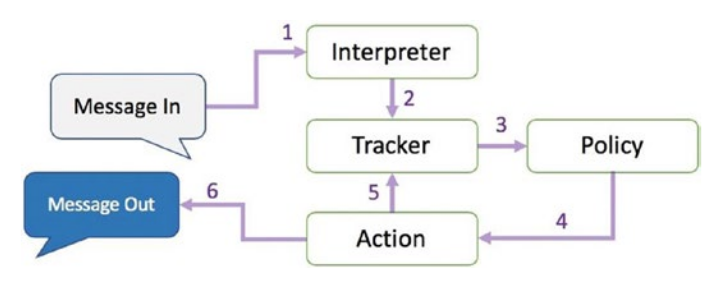
\includegraphics[scale=0.5]{pics/rasa-core}
    \caption{Rasa Core Aufbau~\cite{rasaCoreBook}}
    \label{fig:rasa_core}
\end{figure}

\subsection{Policies}\label{subsec:policies}
\setauthor{Lukas Starka}

Policies sind ein Teil von \textbf{Rasa Core} ~\ref{subsec:rasa-core} und der Assistent benützt Policies um zu entscheiden, welche Action als Nächstes ausgeführt werden soll.
Es gibt machine-learning und rule-based Policies.\cite{policies}

Hierbei können die Policies geändert werden, indem man diese in der \textbf{config.yml} Datei ändert.

Bei den Policies gibt es unterschiedliche Priorities, die dann zum Einsatz kommen, wenn mehrere Policies dieselbe Confidence vorhergesagt haben.\cite{policyPriority}

\subsubsection{TED Policy}
\setauthor{Lukas Starka}

Die TED Policy steht für Transformer Embedding Dialogue Policy und wird meistens standardmäßig verwendet.\cite{tedPolicy}

Bei jedem Dialog bekommt die TED Policy drei Informationen als Input.
Die Nachricht des Users, die vorherige Action, die vorhergesagt wurde und Slots ~\ref{subsec:slots} und aktive Forms ~\ref{subsection:forms}.
Danach wird die Ähnlichkeit zwischen den System Actions und dem eingegebenen Text berechnet und zum Schluss werden noch CRF ~\ref{subsec:crfentityextractor} Algorithmen verwendet, um Entities ~\ref{subsection:entities} zu erkennen.\cite{tedPolicy}

\subsection{Rasa NLU}\label{subsec:rasa-nlu}
\setauthor{Lukas Starka}

Rasa NLU hat grundsätzlich zwei Hauptaufgaben.

Zum einen wäre da die Intent Recognition und die Entity Recognition.\cite{rasanlu, pretrainedVsSupervised}

Die Intent Recognition, ist die Erkennung der Nutzer-Absichten.
Dazu muss das NLU mit ausreichend Utterances, also Responses ~\ref{subsec:Responses} trainiert werden.
Dabei gibt das NLU alle zugehörigen Intents ~\ref{subsec:Intents} geordnet nach dem Confidence Score zurück.
Dieser Score gibt an, wie sicher sich das Modell ist, dass die jeweilige Antwort die richtige Antwort für den Text der Benutzerin oder des Benutzers ist.
Rasa verfügt demnach über ein \textbf{Multi Intent Matching}.\cite{rasanlu, pretrainedVsSupervised}

Außerdem gibt es noch die Entity Recognition, die dafür zuständig ist Entities ~\ref{subsection:entities}, also wichtige Informationen aus natürlicher Sprache zu extrahieren.\cite{rasanlu}

Der Aufbau des NLU ist vollständig konfigurierbar mithilfe der sogenannten Pipeline ~\ref{sec:pipeline}.\cite{howToChooseAPipeline}

\section{Pipeline}\label{sec:pipeline}
\setauthor{Lukas Starka}

Rasa Open Source bietet bei der Initialisierung ~\ref{section:initialize} des Projekts eine Standard-NLU-Konfiguration an.\cite{tuningYourModel}

In Rasa Open Source werden eingehende Nachrichten von einer Reihe von Komponenten ~\ref{sec:components} verarbeitet.
Diese Komponenten werden nacheinander in einer sogenannten Processing Pipeline ausgeführt, die in der \texttt{config.yml} Datei definiert ist.\cite{howToChooseAPipeline}

In der Abbildung ~\ref{fig:component_lifecycle} werden die Komponenten und ihre Lifecycle abgebildet.

\begin{figure}[hbt!]
    \centering
    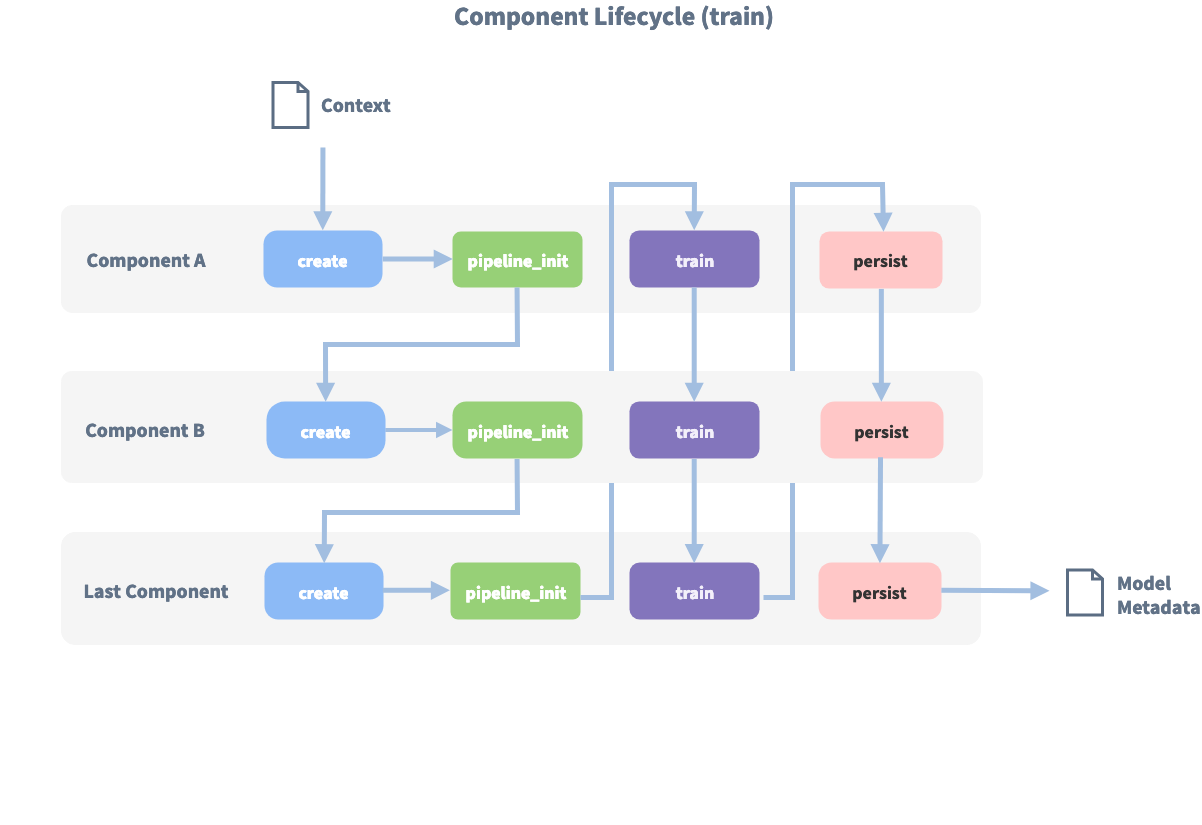
\includegraphics[scale=0.25]{pics/component-lifecycle}
    \caption{Component Lifecycle~\cite{componentLifecycle}}
    \label{fig:component_lifecycle}
\end{figure}

Bevor die erste Komponente mit der Create-Funktion erstellt wird, wird ein sogenannter Kontext erstellt.
Dieser ist ein Python Dictionary, also ein Key-Value-Paar und er wird verwendet, um Informationen zwischen den Komponenten zu übergeben.\cite{componentLifecycle, componentLifecycleDoc}

Zunächst wird der Kontext mit allen Konfigurationswerten gefüllt.
Die Pfeile im Bild ~\ref{fig:pipeline_image} zeigen die Aufrufreihenfolge und visualisieren den Pfad des übergebenen Kontexts.\cite{componentLifecycle, componentLifecycleDoc}
Dies ist in der Grafik ~\ref{fig:pipeline_image} zu erkennen.

\begin{figure}[hbt!]
    \centering
    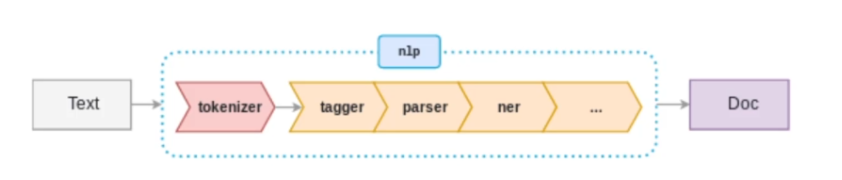
\includegraphics[scale=0.5]{pics/pipeline}
    \caption{Component Lifecycle~\cite{pipelineImage}}
    \label{fig:pipeline_image}
\end{figure}

\subsection{Arten von NLU Pipelines}\label{subsec:pipeline-types}
\setauthor{Lukas Starka}

Es gibt verschiedene bereits konfigurierte Pipelines.\cite{howToChooseAPipeline}

Grundsätzlich ist zwischen Pipelines mit oder ohne Pretrained Word Vectors zu unterscheiden.

\subsubsection{Beispiele für Pipelines mit Pretrained Word Vectors}

Der Vorteil von Pipelines, die Pretrained Word Vectors verwenden ist, dass diese bereits aus der jeweiligen Sprache Vektoren für die Wörter besitzen.
Somit weiß das Modell beispielsweise, dass Äpfel und Birnen ähnlich sind, ohne dass dies in den Intents irgendwo spezifiziert werden muss, weil es bereits aus den Wordvektoren hervorgeht.\cite{differenceStackOverflow, rasaMasterclassPreConfiguredPipelines}

Die Vorteile hierbei sind also, dass das Modell weniger Trainingsdaten benötigt, um eine gute Leistung zu erzielen.
Außerdem ist der Trainingsprozess in der Regel schneller und die Zeit, die benötigt wird, um die Trainingsdaten zu durchlaufen, ist kürzer als bei Modellen ohne Pretrained Word Vectors.\cite{differenceStackOverflow, pretrainedVsSupervised, rasaMasterclassPreConfiguredPipelines}
Ein Beispiel für eine Pipeline mit vortrainierten Vektoren ist die \texttt{spacy\_sklearn} Pipeline, die man in der \texttt{config.yml} Datei wie in Listing ~\ref{lst:spacy-sklearn-pipeline} definiert.

\begin{lstlisting}[label={lst:spacy-sklearn-pipeline},caption={SpaCy Sklearn Pipeline}]{SpaCy Sklearn Pipeline}
language: "de"

pipeline: "spacy_sklearn"
\end{lstlisting}

Die SpaCy Pipeline verwendet Pretrained Word Vectors von GloVe oder fastText.
Dies sind Algorithmen, die einen Textkorpus ~\ref{subsec:corpus} einer gewissen Sprache in Form von Vektoren einarbeiten.\cite{spacySklearnPipeline, spacyNLP, rasaMasterclassPreConfiguredPipelines}

Es gibt außerdem auch noch Pipelines von MITIE.
Diese verwenden MITIE als Source für die Word Vectors.
Ein Vorteil von MITIE ist, dass man hier auch seine eigenen Word Vectors trainieren kann, indem man einen Korpus ~\ref{subsec:corpus} von Wikipedia oder ähnlichen Seiten verwendet.
Allerdings wird MITIE meistens nicht empfohlen und es könnte auch sein, dass MITIE demnächst deprecated sein wird.
Die MITIE Pipeline kann man wie in Listing ~\ref{lst:mitie-sklearn-pipeline} definieren.\cite{mitieNLP, mitieDeprecated}

\begin{lstlisting}[label={lst:mitie-sklearn-pipeline},caption={MITIE Sklearn Pipeline}]{MITIE Sklearn Pipeline}
language: "de"

pipeline: "mitie_sklearn"
\end{lstlisting}

\subsubsection{Beispiele für Pipelines ohne Pretrained Word Vectors}\label{subsubsec:pipeline-without-pretrained-word-vectors}

Der Vorteil von Pipelines ohne Pretrained Word Vectors ist, dass diese speziell auf den Fachbereich angepasst sind, für den man den Chatbot entwickelt.\cite{pretrainedVsSupervised, tensorFlowEmbedding}

Als Beispiel kann man die Wörter \texttt{balance} und \texttt{symmetry} aus dem Englischen sehen.
Diese Wörter sind eng miteinander verwandt.
Allerdings kann im Kontext von Banken das Wort \texttt{balance} auch mit \texttt{cash} verwandt sein.
Bei einem vortrainierten Modell würden diese Wortvektoren nicht nah aneinander liegen, aber wenn ein Chatbot nur Intents besitzt, die mit Banken und Rechnungswesen zu tun haben, werden diese zwei Wörter \texttt{balance} und \texttt{cash} ohne Pretrained Word Vectors auch als ähnlich erkannt werden.\cite{tensorFlowEmbedding}

Außerdem benutzen diese Pipelines kein sprach-spezifisches Modell und somit kann man sie in allen Sprachen verwenden, die tokenisiert werden können.
Eine solche Pipeline kann man wie in Listing ~\ref{lst:tensorflow-embedding-pipeline} definieren.\cite{tensorFlowEmbedding}

\begin{lstlisting}[label={lst:tensorflow-embedding-pipeline},caption={Tensorflow Embedding Pipeline}]{Tensorflow Embedding Pipeline}
language: "de"

pipeline: "tensorflow_embedding"
\end{lstlisting}

Ein Problem von diesem Ansatz ist jedoch, dass er oftmals keine fachspezifischen Begriffe kennt und außerdem können Typos nicht als Wortvektoren gelernt werden.
Außerdem ist das Problem bei Pretrained Word Vectors, dass Zehntausende Vektoren gespeichert werden, die vermutlich nie verwendet werden.\cite{tensorFlowEmbedding, choosingPipeline}

Das Tensorflow-Embedding ist das genaue Pendant dazu.
Diese Pipeline verwendet keine vortrainierten Vektoren und kann mit jeder Sprache verwendet werden.
Sie lernt dabei Embeddings für die Intents ~\ref{subsec:Intents} und für die Wörter einer Sprache.
Diese Embeddings werden verwendet, um die Ähnlichkeit zwischen dem Input und den Intents ~\ref{subsec:Intents} zu ermitteln.\cite{tensorFlowEmbedding, choosingPipeline}

Eine solche Pipeline wird wie in Listing ~\ref{lst:supervised-embedding} definiert.

\begin{lstlisting}[label={lst:supervised-embedding},caption={Supervised Embedding Pipeline}]{Supervised Embedding Pipeline}
language: "de"

pipeline: "supervised_embedding"
\end{lstlisting}

\subsubsection{Supervised Embeddings vs. Pretrained Embeddings}\label{subsubsec:supervised-embedding-vs-pretrained-embedding}

In der Grafik ~\ref{fig:pre_trained_vs_supervised} ist ein Flussdiagramm abgebildet, welches beschreibt, wann Supervised Embeddings oder Pretrained Embeddings von Vorteil sind.

\begin{figure}[hbt!]
    \centering
    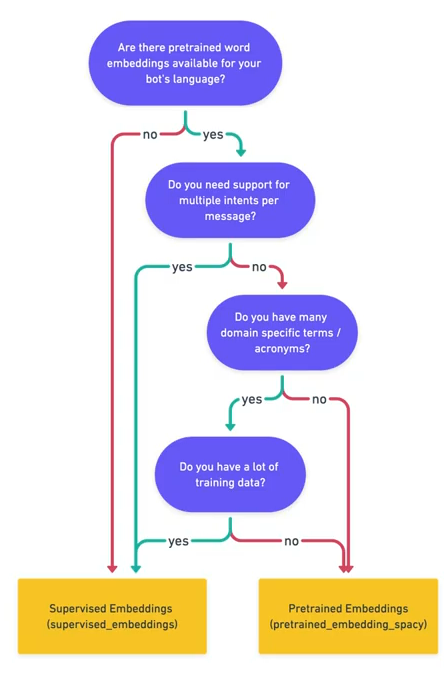
\includegraphics[scale=0.5]{pics/pre-trained-vs-supervised}
    \caption{Pretrained oder Supervised Embeddings~\cite{pretrainedVsSupervised, rasaMasterclassPreConfiguredPipelines}}
    \label{fig:pre_trained_vs_supervised}
\end{figure}

\subsection{Konfigurierte Pipelines}\label{subsec:configured-pipelines}
\setauthor{Lukas Starka}

Es gibt vordefinierte Pipelines von Rasa, die benutzt werden können.

Sollte man sich für Word Embeddings entscheiden, kann man auf eine Pipeline mit SpaCy zurückgreifen, welche den SpacyFeaturizer verwendet und somit Pretrained Word Embeddings nutzt.
Diese ist in Listing ~\ref{lst:spacy-pipeline} zu sehen.\cite{startingPipelines, allComponents}

\begin{lstlisting}[label={lst:spacy-pipeline},caption={Spacy Startpipeline}]{Spacy Startpipeline}
language: "de"  # Code für die Sprache

pipeline:
  - name: SpacyNLP
    model: "de_core_news_lg" # Spezifizierung, welches Modell von SpaCy genommen werden soll
  - name: SpacyTokenizer
  - name: SpacyFeaturizer
  - name: RegexFeaturizer
  - name: LexicalSyntacticFeaturizer
  - name: CountVectorsFeaturizer
  - name: CountVectorsFeaturizer
    analyzer: "char_wb"
    min_ngram: 1
    max_ngram: 4
  - name: DIETClassifier
    epochs: 100
  - name: EntitySynonymMapper
  - name: ResponseSelector
    epochs: 100

\end{lstlisting}

Wenn man sich dafür entscheidet, keine vortrainierten Word Embeddings zu nutzen und somit sein Modell spezifischer auf den eigenen Anwendungsfall anpassen möchte, verwendet man die vordefinierte Rasa Pipeline.
Diese verwendet den CountVectorsFeaturizer.
Bei diesem werden nur die Trainingsdaten, die zur Verfügung gestellt werden, trainiert.\cite{startingPipelines, allComponents, nluExamples}
In der \texttt{config.yml} Datei würde die Pipeline somit wie in Listing ~\ref{lst:default-pipeline} aussehen.

\begin{lstlisting}[label={lst:default-pipeline},caption={Default Pipeline}]{Default Pipeline}
language: "de"  # Code für die Sprache

pipeline:
  - name: WhitespaceTokenizer
  - name: RegexFeaturizer
  - name: LexicalSyntacticFeaturizer
  - name: CountVectorsFeaturizer
  - name: CountVectorsFeaturizer
    analyzer: "char_wb"
    min_ngram: 1
    max_ngram: 4
  - name: DIETClassifier
    epochs: 100
  - name: EntitySynonymMapper
  - name: ResponseSelector
    epochs: 100

\end{lstlisting}

\subsection{Verwendete Pipeline}\label{subsec:our-pipeline}
\setauthor{Lukas Starka}

Die für die Umsetzung des Chatbots verwendete Pipeline aus Listing ~\ref{lst:our-pipeline} beruht dabei auf dieser Standard-Pipeline.
In den folgenden Kapiteln werden diese Komponenten davon genauer erläutert.

\begin{lstlisting}[label={lst:our-pipeline},caption={Unsere Pipeline}]{Unsere Pipeline}
language: de

pipeline:
   - name: WhitespaceTokenizer
   - name: RegexFeaturizer
   - name: LexicalSyntacticFeaturizer
   - name: CountVectorsFeaturizer
   - name: CountVectorsFeaturizer
     analyzer: char_wb
     min_ngram: 1
     max_ngram: 4
   - name: DIETClassifier
     epochs: 100
     constrain_similarities: true
   - name: EntitySynonymMapper
   - name: ResponseSelector
     epochs: 100
     retrieval_intent: faq
   - name: ResponseSelector
     epochs: 100
     retrieval_intent: chitchat
   - name: FallbackClassifier
     threshold: 0.3
     ambiguity_threshold: 0.1
\end{lstlisting}

\subsection{Pipelines vergleichen}\label{subsec:comparing-pipelines}
\setauthor{Lukas Starka}

Um die beste Leistung für definierte Trainingsdaten zu erzielen, gibt es die Möglichkeit, zwei verschieden Pipelines miteinander zu vergleichen.
Dafür wird der \texttt{rasa test} Befehl verwendet, der dabei eine Reihe von verschiedenen Schritten ausführt, wie in Listing ~\ref{lst:comparing-pipelines} zu sehen ist.
gibt es
\begin{enumerate}
    \item Zunächst werden 80 \% der Daten von der \texttt{data/nlu.yml} Datei trainiert und 20 \% getestet.
    \item Danach wird eine gewisse Prozentzahl von Daten ausgelassen.
    \item Die Modelle werden basierend auf den überbleibenden Daten trainiert.
    \item Eine Evaluation über das Modell mit den reduzierten Trainingsdaten wird erstellt.\cite{comparingNLUPipelines}
\end{enumerate}

Der zweite Schritt wird dabei standardmäßig dreimal für jede übergebene Pipeline-Konfiguration ausgeführt.
Dabei werden immer wieder neue Prozentzahlen gewählt.
Um diese zu verändern, gibt es die \texttt{--runs} Flag, die in Listing ~\ref{lst:comparing-pipelines-custom} zu sehen ist.\cite{comparingNLUPipelines}

\begin{lstlisting}[label={lst:comparing-pipelines},caption={Unsere Pipeline}]{Unsere Pipeline}
rasa test nlu --nlu data/nlu.yml
   --config config_1.yml config_2.yml
\end{lstlisting}

\begin{lstlisting}[label={lst:comparing-pipelines-custom},caption={Unsere Pipeline}]{Unsere Pipeline}
rasa test nlu --nlu data/nlu.yml
  --config config_1.yml config_2.yml
  --runs 4 --percentages 0 25 50 70 90
\end{lstlisting}

\subsubsection{Evaluation der Ergebnisse}\label{subsubsec:evaluation-results}
\setauthor{Lukas Starka}

Nachdem nun ein ausführlicher Test aller NLU-Daten durchgeführt wurde, wird das Ergebnis in einem \texttt{results/} Ordner gespeichert.\cite{interpretingTheOutput}

Dort befindet sich nun direkt im Ordner eine Datei mit den Ergebnissen der verglichenen Pipelines.
In der Abbildung ~\ref{fig:comparision_graph} ist zu erkennen, dass hierbei nur ein Konfigurationsfile getestet wurde.
Bei diesem handelt es sich um die im Zuge der Arbeit gewählte Pipeline.
Auf der x-Achse befindet sich die Anzahl der Trainingsphrasen, die beim Training dabei waren.
Hier ist zu sehen, dass je höher die Anzahl ist, desto genauer auch der F1-Score ~\ref{subsec:F-Score} ist.
Vor allem aber sind die Abweichungen bei diesem Score viel kleiner, wenn mehr Trainingsphrasen gegeben sind.
Dies beweist, wie wichtig es ist, viele Trainingsphrasen zu verwenden.

\begin{figure}[hbt!]
    \centering
    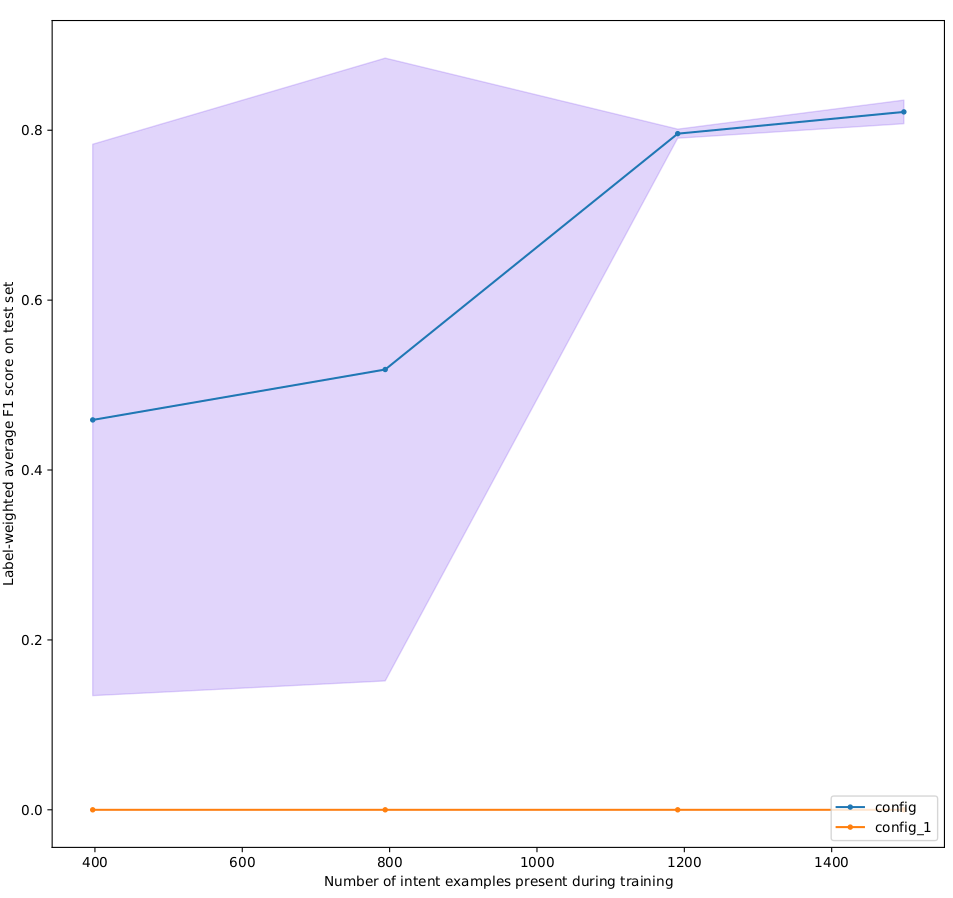
\includegraphics[scale=0.4]{pics/comparision_graph}
    \caption{Comparision Graph bei unserer Pipeline}
    \label{fig:comparision_graph}
\end{figure}

Außerdem werden noch \texttt{.json}-Dateien und Bilder für die Ergebnisse erzeugt.
Für jeden Lauf wird hierbei ein Ordner angelegt, in dem es Unterordner für die jeweilige Prozentzahl gibt, die von den Trainingsphrasen ausgeschlossen wurde.
Dabei findet sich jeweils eine sogenannte Konfusionsmatrix und ein Histogramm der Ergebnisse.

Beim Histogramm wird die Anzahl der korrekt vorhergesagten Intents ~\ref{subsec:Intents} mit der von den falsch vorhergesagten Intents ~\ref{subsec:Intents} verglichen.
Dabei wird auch die Confidence, also die Sicherheit des Modells, angegeben, mit der sie vorhergesagt wurden.
Im Optimalfall sind die Balken also bei den korrekten Intents weit oben mit einer hohen Confidence versehen und die Falschen mit einer niedrigen.
Außerdem soll die Anzahl, die auf der x-Achse eingetragen ist, von den richtigen Intents höher sein als die Anzahl der falschen Intents.
In Abbildung ~\ref{fig:histogram_0} ist ein Histogramm für 0\% Exklusion zu sehen und bei Abbildung ~\ref{fig:histogram_75} wurde 75\% Exklusion genutzt.
Es ist dabei zu erkennen, dass bei mehr Exklusion auch mehr Intents ~\ref{subsec:Intents} falsch vorhergesagt werden und die Zuversichtlichkeit, also die Confidence, des Modells dabei immer höher wird.

\begin{figure}[hbt!]
    \centering
    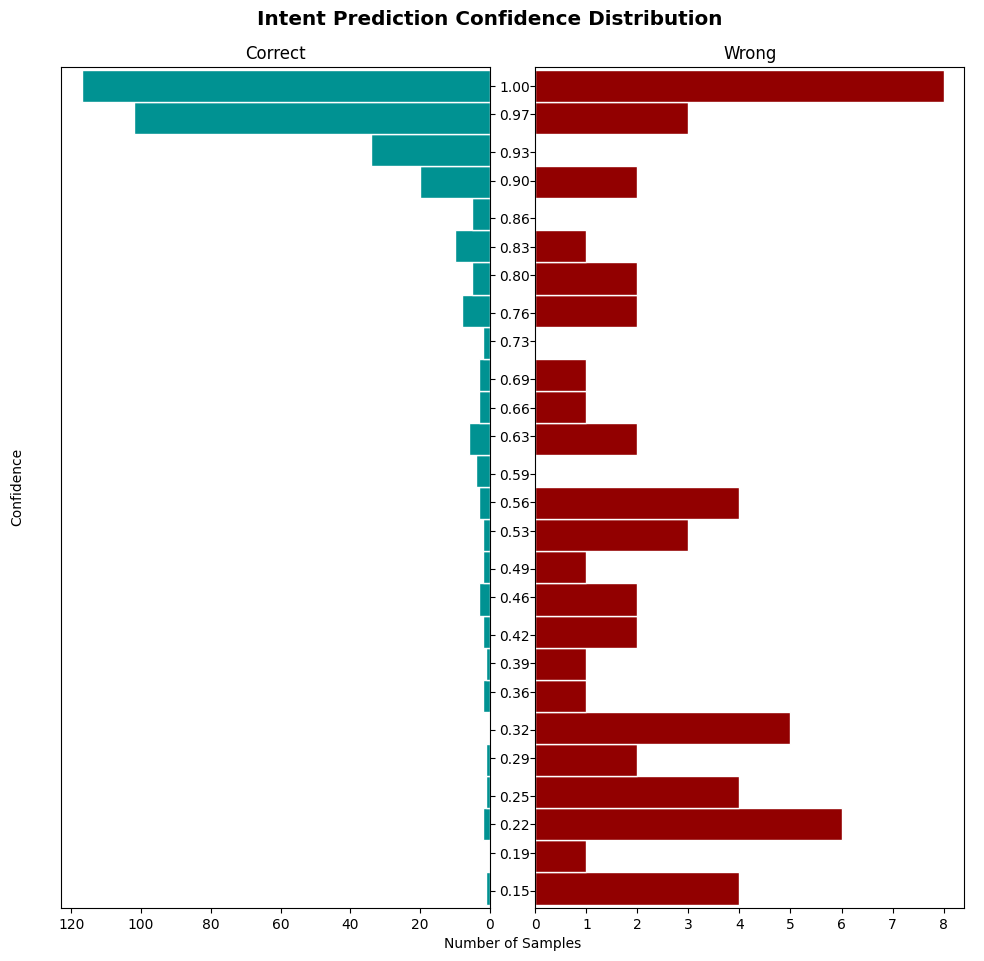
\includegraphics[scale=0.5]{pics/intent_histogram_0}
    \caption{Histogramm für 0\% Exklusion}
    \label{fig:histogram_0}
\end{figure}

\begin{figure}[hbt!]
    \centering
    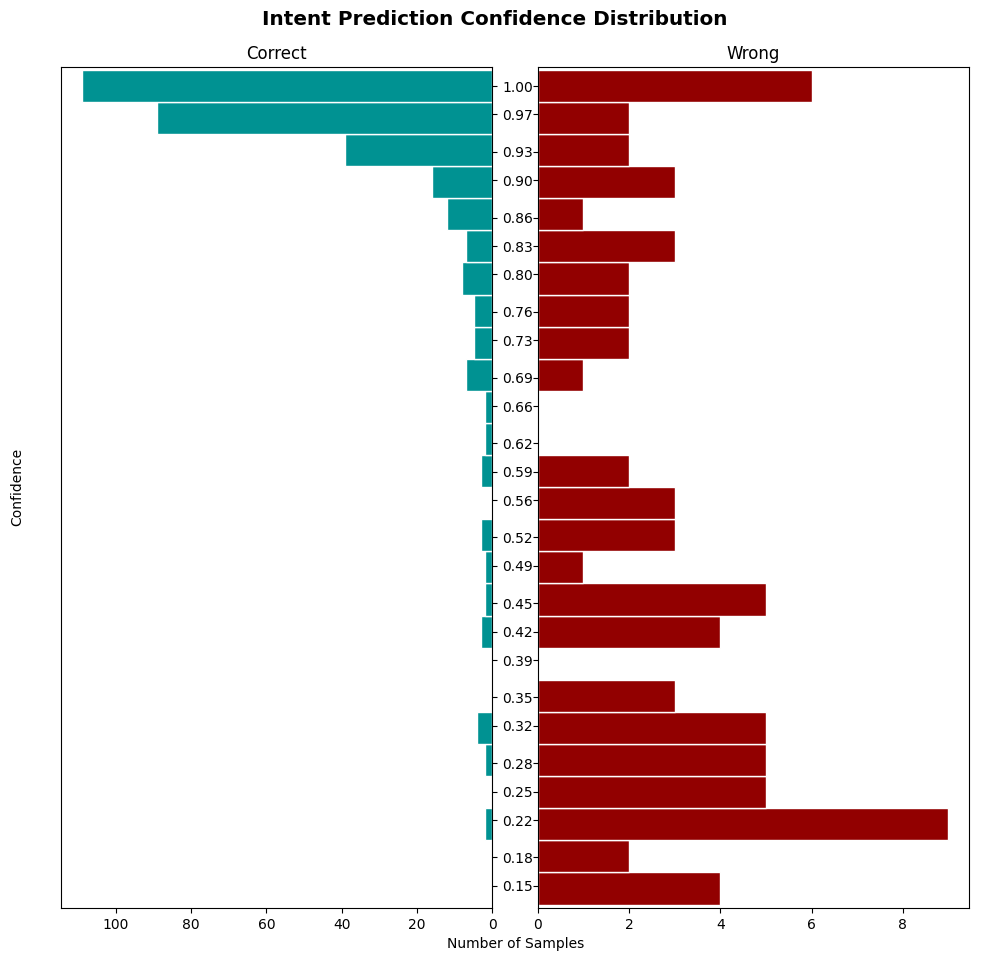
\includegraphics[scale=0.5]{pics/intent_histogram_75}
    \caption{Histogramm für 75\% Exklusion}
    \label{fig:histogram_75}
\end{figure}

Die Konfusionsmatrix hilft dabei festzustellen, wie viele Intents richtig und falsch erkannt wurden.
Dabei wird auf einer Achse aufgetragen, welcher Intent vorhergesagt wurde und welcher Intent tatsächlich erkannt hätte werden sollen.
Im Optimalfall liegt bei der Konfusionsmatrix also eine Diagonale durch die Matrix vor.
Bei der Konfusionsmatrix ist anschaulich zu erkennen, welche Intents noch überarbeitet werden sollten, weil zu viele Intents falsch als dieser vorhergesagt wurden.
In Abbildung ~\ref{fig:confusion_matrix} kann man beispielsweise ablesen, dass zwei Intents, die eigentlich \texttt{chitchat/insult} sein sollten fälschlicherweise als \texttt{chitchat/ask\_creator} erkannt wurden.

\begin{figure}[hbt!]
    \centering
    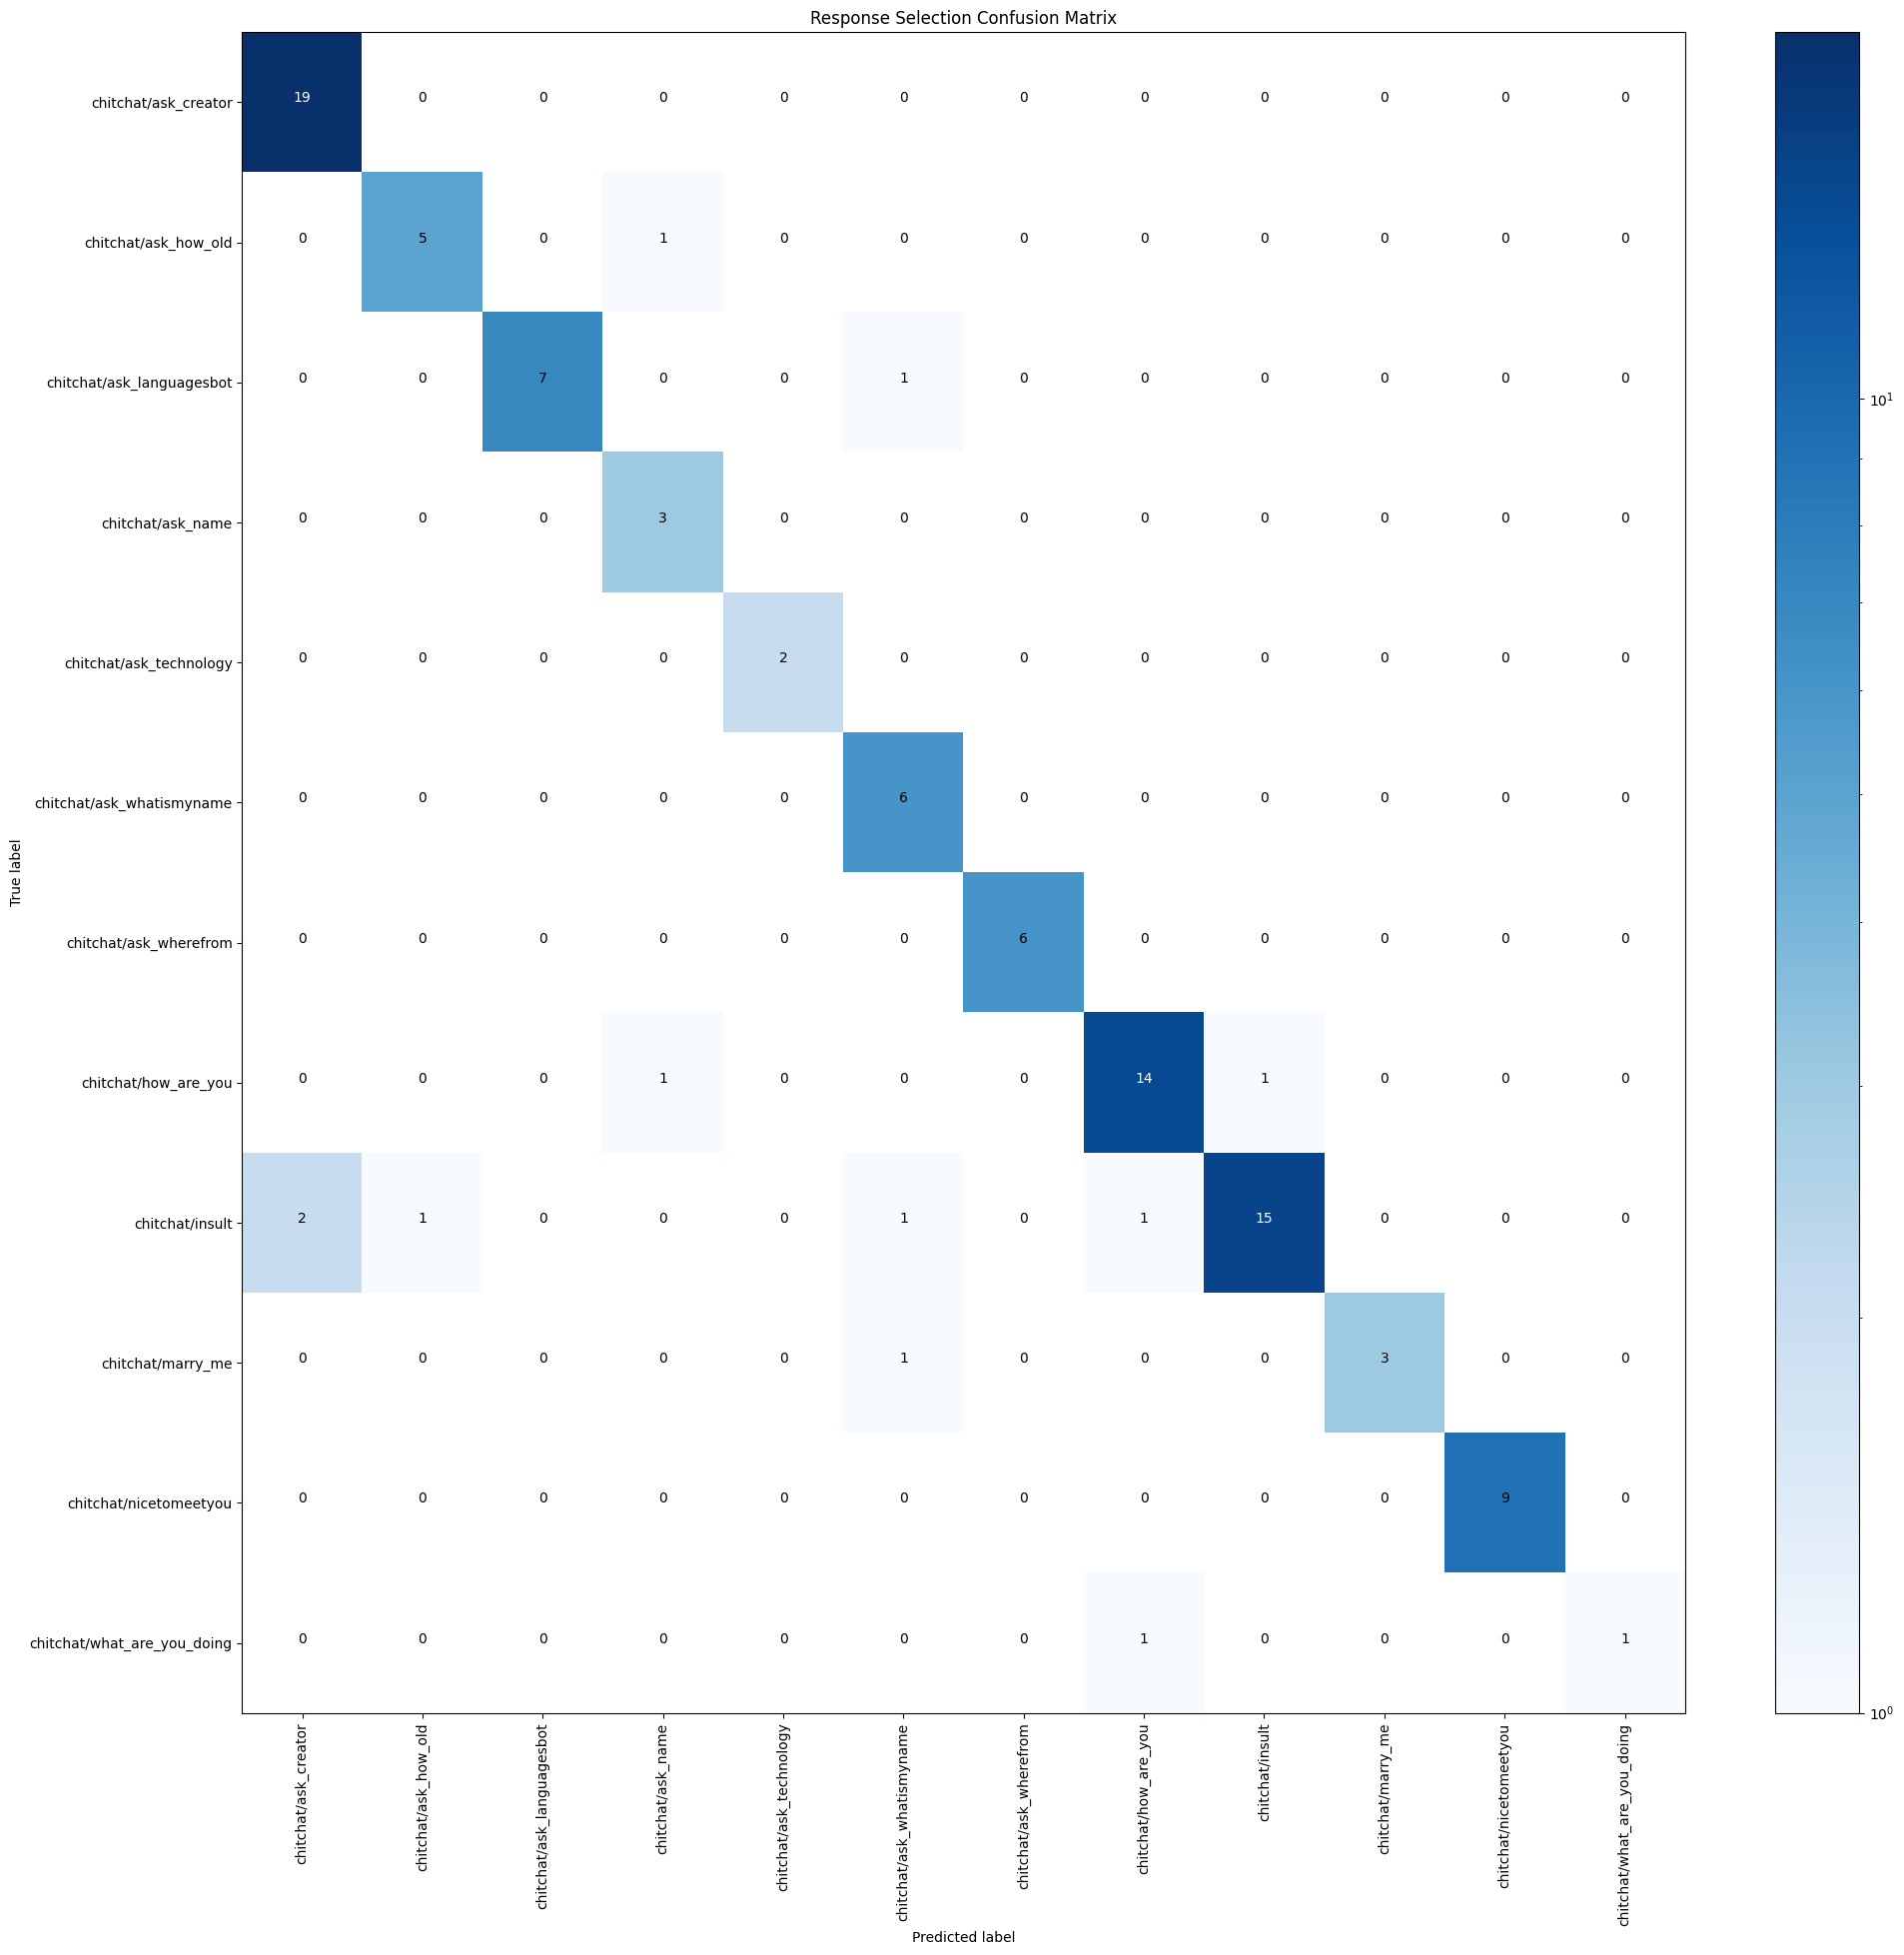
\includegraphics[scale=0.3]{pics/confusion_matrix}
    \caption{Konfusionsmatrix für chitchat Intents}
    \label{fig:confusion_matrix}
\end{figure}

\subsection{WhitespaceTokenizer}\label{subsec:whitespace-tokenizer}
\setauthor{Lukas Starka}

Ein WhitespaceTokenizer ist eine sehr einfache Art eines Tokenizers.
Hierbei wird, wie der Name bereits vermuten lässt, der Satz aufgeteilt in verschiedene Tokens.
Ein Token kann beispielsweise ein Wort sein und beim WhitespaceTokenizer wird der Satz pro Whitespace, also pro Leerzeichen, aufgeteilt.\cite{whitespaceTokenizer, rasaMasterclassWhitespaceTokenizer, pipelineComponentsYoutube}

\begin{figure}[hbt!]
    \centering
    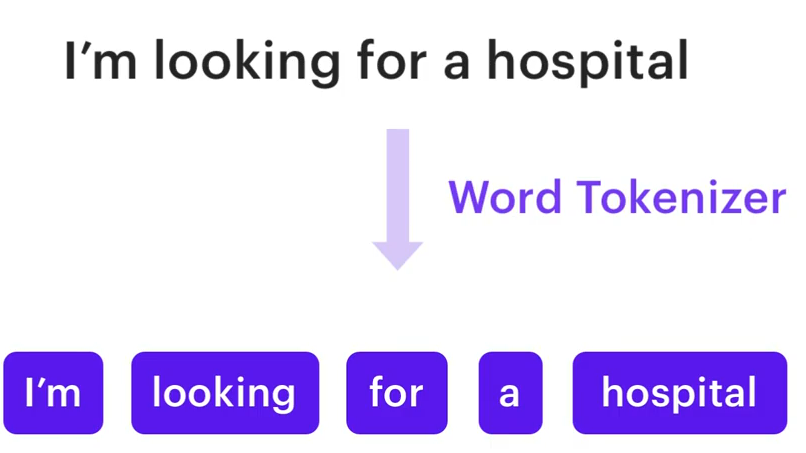
\includegraphics[scale=0.25]{pics/whitespacetokenizer}
    \caption{Tokens durch einen WhitespaceTokenizer~\cite{pipelineComponentsYoutube}}
    \label{fig:WhitespaceTokenizer}
\end{figure}

Es gibt auch komplexere Tokenizer und Tokenizer, die speziell an Sprachen angepasst sind und die besonderen Regeln, die in diesen Sprachen gelten, beachten.
Außerdem kann ein Tokenizer auch selber implementiert werden.\cite{whitespaceTokenizer, rasaMasterclassWhitespaceTokenizer, pipelineComponentsYoutube}
Tokenizer sollten generell weit am Anfang einer Pipeline ~\ref{sec:pipeline}, wenn nicht sogar die erste Komponente sein.

\subsection{RegexFeaturizer}\label{subsec:regex-featurizer}
\setauthor{Lukas Starka}

Einen RegexFeaturizer kann man verwenden, um die EntityExtraction zu erleichtern.
Bei diesem werden Regular Expressions ~\ref{subsubsec:regex-featurizer-regex} und Lookup Tables ~\ref{subsubsec:lookup-tables} verwendet und der RegexFeaturizer gibt an, ob ein Wort von den Regular Expressions oder Lookup Tables erkannt wurde.\cite{rasaMasterclassRegexFeaturizer, pipelineComponentsYoutube, regexFeaturizerCrf}

\subsubsection{Regular Expressions}\label{subsubsec:regex-featurizer-regex}

Regular Expressions können verwendet werden, um Muster eines Strings zu beschreiben und können hier bei dem Beispiel von Chatbots verwendet werden, um Zahlen zu beschreiben, wie in Abbildung ~\ref{fig:Regular Expression Beispiel} zu sehen ist.\cite{rasaMasterclassRegexFeaturizer, pipelineComponentsYoutube, regexFeaturizerCrf}

\begin{figure}[hbt!]
    \centering
    
\includegraphics[scale=0.5]{pics/regular-expression-example}
    \caption{Regular Expression Beispiel~\cite{pipelineComponentsYoutube}}
    \label{fig:Regular Expression Beispiel}
\end{figure}

\subsubsection{Lookup Tables}\label{subsubsec:lookup-tables}

Lookup Tables können verwendet werden, wenn eine Entity vordefinierte Werte haben kann.
Zum Beispiel kann eine Entity mit dem Namen \texttt{country} 194 verschiedene Länder annehmen.\cite{rasaMasterclassRegexFeaturizer, pipelineComponentsYoutube, regexFeaturizerCrf}

\begin{figure}[hbt!]
    \centering
    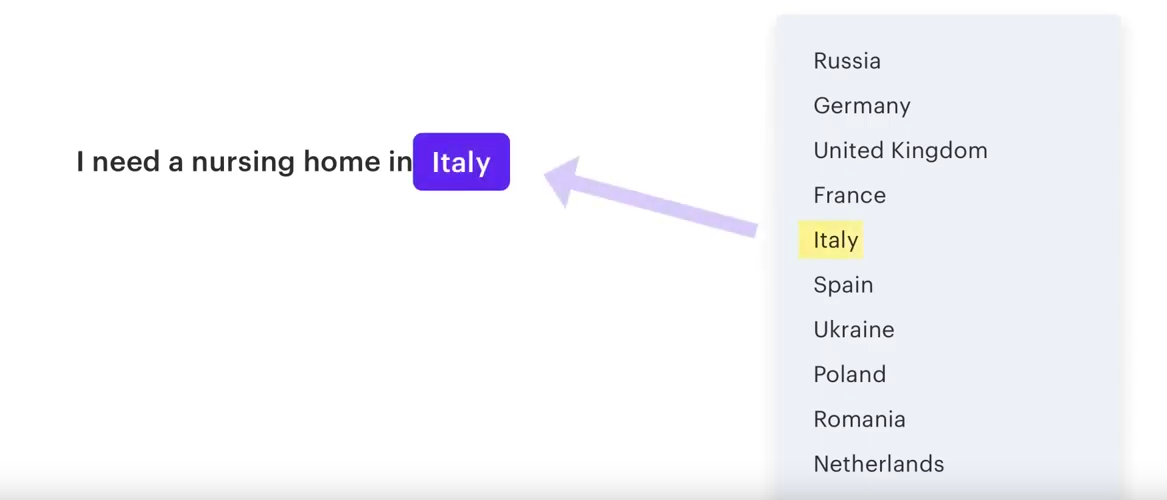
\includegraphics[scale=0.25]{pics/lookup-table-example}
    \caption{Lookup Table Beispiel~\cite{pipelineComponentsYoutube}}
    \label{fig:Lookup Table Beispiel}
\end{figure}

Der RegexFeaturizer muss vor dem EntityExtractor in der Pipeline platziert werden.\cite{rasaMasterclassRegexFeaturizer, pipelineComponentsYoutube, regexFeaturizerCrf}

\subsection{CRFEntityExtractor}\label{subsec:crfentityextractor}
\setauthor{Lukas Starka}

Eine Möglichkeit, um Entities ~\ref{subsection:entities} aus der Nachricht des Benutzers zu extrahieren ist über den CRFEntityExtractor.\cite{crfEntityExtractor}

CRF steht hierbei für Conditional Random Field.
Dieses Modell lernt, welche Komponenten eines Satzes Entities sind und welche Entities diese sind.\cite{crfEntityExtractor, pipelineComponentsYoutube, regexFeaturizerCrf}

Dies macht der CRFEntityExtractor, indem er die Sequenzen der Tokens beobachtet.
Es wird also ein Token aus dem Satz ausgewählt, und anschließend wird geschaut, ob die Wörter danach und davor zum Kontext des Wortes beitragen, um zu erkennen, ob es sich hierbei um eine Entity handelt.
Dabei schaut der Extractor auf Eigenschaften, wie beispielsweise, ob das Wort groß- oder kleingeschrieben ist, ob es einen Präfix hat, ob es eine Zahl ist oder ob es ein speziell definiertes Wort für die Entities ist.
Dies wird auch mit den Wörtern davor und danach gemacht.\cite{crfEntityExtractor, pipelineComponentsYoutube, regexFeaturizerCrf}

\begin{figure}[hbt!]
    \centering
    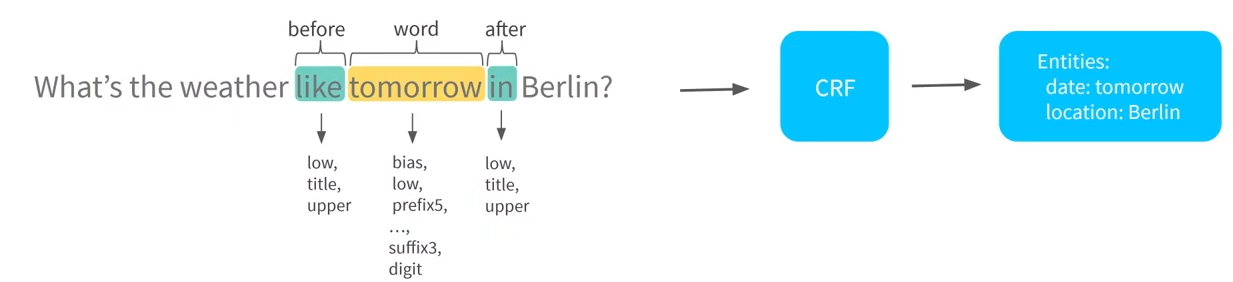
\includegraphics[scale=0.35]{pics/crf-entity-extractor}
    \caption{Funktionsweise vom CRFEntityExtractor~\cite{pipelineComponentsYoutube}}
    \label{fig:CRFEntityExtractor}
\end{figure}

Der CRFEntityExtractor produziert anschließend als Output, welche Wörter in einem Satz Entities sind und welche Entities diese sind, also was ihre Labels sind.
Außerdem wird noch produziert, wie sicher das Modell war, dass diese Entities korrekt sind, also wird die sogenannte Confidence ausgegeben und welches Modell verwendet wurde.\cite{crfEntityExtractor, pipelineComponentsYoutube, regexFeaturizerCrf}

\subsection{LexicalSyntacticFeaturizer}\label{subsec:lexical-syntactic-featurizer}
\setauthor{Lukas Starka}

Ein Featurizer wird generell verwendet, um Features von den Tokens zu extrahieren.
Diese können dann von dem Intent-Klassifikations-Modell genutzt werden, um Muster zu erkennen und anschließend den korrekten Intent ~\ref{subsec:Intents} vorherzusagen.\cite{lexicalSyntacticFeaturizer, pipelineComponentsYoutube, pipelineConfigurationVideo}

\begin{figure}[hbt!]
    \centering
    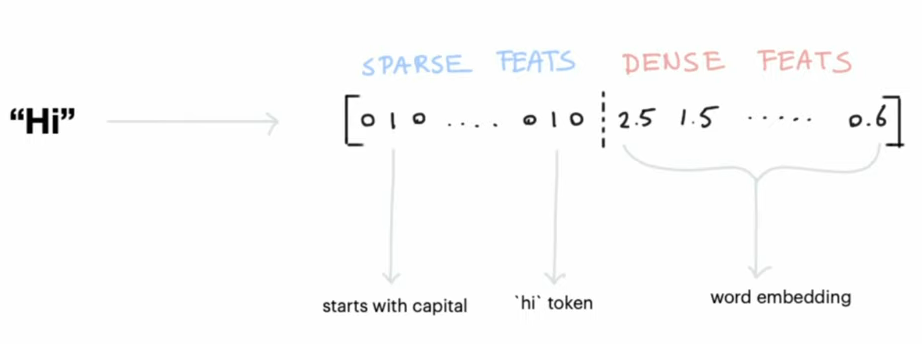
\includegraphics[scale=0.5]{pics/featurizer}
    \caption{Funktionsweise von einem Featurizer~\cite{pipelineConfigurationVideo}}
    \label{fig:Featurizer}
\end{figure}

\subsection{CountVectorsFeaturizer}\label{subsec:count-vectors-featurizer}
\setauthor{Lukas Starka}

Der CountVectorsFeaturizer erstellt Bag-of-Words ~\ref{subsec:bag-of-words}.
Dabei wird gezählt, wie oft ein bestimmtes Wort aus den Trainingsdaten in der Nachricht des Benutzers vorkommt.\cite{countVectorsFeaturizer, pipelineConfigurationVideo, pipelineComponentsYoutube, rasaMasterclassCountVectorsFeaturizer}

\begin{figure}[hbt!]
    \centering
    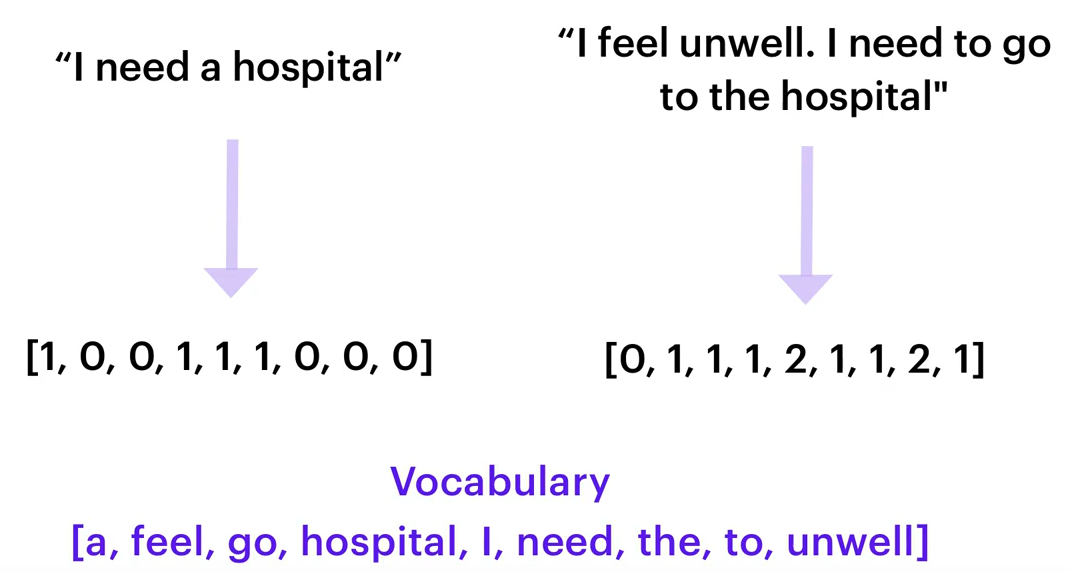
\includegraphics[scale=0.25]{pics/countvectorsfeaturizer}
    \caption{CountVectorsFeaturizer Beispiel~\cite{pipelineConfigurationVideo}}
    \label{fig:CountVectorsFeaturizer}
\end{figure}

Beim CountVectorsFeaturizer kann außerdem angeben werden, dass statt Wörtern sogenannte n-grams ~\ref{subsec:bag-of-ngrams} verwendet werden sollen.
Dies macht das Modell in der Regel robuster gegen Typos allerdings erhöht sich damit auch die Zeit, die das Modell zum Trainieren benötigt.\cite{countVectorsFeaturizer, pipelineConfigurationVideo, pipelineComponentsYoutube, rasaMasterclassCountVectorsFeaturizer}

\begin{lstlisting}[label={lst:count-vectors-featurizer},caption={CountVectorsFeaturizer}]{CountVectorsFeaturizer}
pipeline:
    - name: CountVectorsFeaturizer
    analyzer: char_wb
    min_ngram: 1
    max_ngram: 4
\end{lstlisting}

\subsection{DIETClassifier}\label{subsec:dietclassifier}
\setauthor{Lukas Starka}

DIET steht für \textbf{Dual Intent and Entity Transformer} und kann somit sowohl Intents ~\ref{subsec:Intents} als auch Entities ~\ref{subsection:entities} klassifizieren und erkennen.
Bei der Klassifizierung wird die Eingabe des Users hergenommen und dabei der passende Intent aus der \texttt{nlu.yml} Datei gefunden.
Ohne DIET würde zusätzlich zur Intent-Klassifizierung auch noch eine Komponente benötigt werden, die Entities extrahiert, wie beispielsweise den CRFEntityExtractor ~\ref{subsec:crfentityextractor}.
Der Parameter \texttt{epochs} gibt dabei an, wie oft die Trainingsdaten durchgegangen werden sollen.
Standardmäßig ist dieser auf den Wert 300 gesetzt.
Je kleiner diese Nummer also ist, desto schneller wird das Modell trainiert.\cite{dietClassifier}

\begin{lstlisting}[label={lst:dietclassifier-pipeline},caption={DietClassifier in Pipeline}]{DietClassifierPipeline}
pipeline:
    - name: DIETClassifier
    epochs: 100
\end{lstlisting}

Der Output des DIETClassifier kann wie in Listing ~\ref{lst:dietclassifier-output} aussehen.
Dabei wird zunächst der Intent angeführt, der mit der höchsten Wahrscheinlichkeit (Confidence) vorhergesagt wurde.
Alle anderen Intents, die das Modell in Betracht gezogen hat, werden nach ihrer Confidence absteigend sortiert ausgegeben.
Zusätzlich sind noch alle Entities, die erkannt wurden, mit deren Wert angeführt, inklusive der Stelle in der Eingabe des Users, an der die jeweiligen Entities erkannt wurden.

\begin{lstlisting}[label={lst:dietclassifier-output},caption={Output des DIETClassifiers ~\cite{dietClassifier}}]{DietClassifierOutput}
{
    "intent": {"name": "greet", "confidence": 0.8343},
    "intent_ranking": [
        {
            "confidence": 0.385910906220309,
            "name": "goodbye"
        },
        {
            "confidence": 0.28161531595656784,
            "name": "restaurant_search"
        }
    ],
    "entities": [{
        "end": 53,
        "entity": "time",
        "start": 48,
        "value": "2017-04-10T00:00:00.000+02:00",
        "confidence": 1.0,
        "extractor": "DIETClassifier"
    }]
}
\end{lstlisting}

\subsection{EntitySynonymMapper}\label{subsec:entitysynonymmapper}
\setauthor{Lukas Starka}

Der EntitySynonymMapper erwartet als Input einen Extractor von den verschiedenen Entity Extraktoren und liefert als Ausgabe modifizierte Werte für die Entities, die bereits vorher erkannt wurden.
Wenn beim EntitySynonymMapper also eine Entity überliefert wird und in den Trainingsdaten Synonyme für diese Entity vorhanden sind, wird der Wert der Entity auf den Wert, der in den Trainingsdaten angegeben ist, gesetzt.
Wenn also beispielsweise in einem Satz des Benutzers New York City oder NYC vorkommt, werden diese beide auf denselben Wert nyc gesetzt.\cite{entitySynonymMapper}

\begin{lstlisting}[label={lst:entity-synonym-mapper},caption={Entity Synonym Mapper}]{Entity Synonym Mapper}
[
    {
      "text": "I moved to New York City",
      "intent": "inform_relocation",
      "entities": [{
        "value": "nyc",
        "start": 11,
        "end": 24,
        "entity": "city",
      }]
    },
    {
      "text": "I got a new flat in NYC.",
      "intent": "inform_relocation",
      "entities": [{
        "value": "nyc",
        "start": 20,
        "end": 23,
        "entity": "city",
      }]
    }
]
\end{lstlisting}

\subsection{ResponseSelector}\label{subsec:response-selector}
\setauthor{Lukas Starka}

Ein Selector sagt die korrekte Response ~\ref{subsec:Responses} aus einer Menge von möglichen Responses voraus.
Beim ResponseSelector wird als Ausgabe ein Key-Value Paar ausgegeben.
Als Key wird hierbei der Retrieval Intent ausgegeben und das Value ist die vorhergesagte Response und die Confidence, mit der diese vorhergesagt wurde.\cite{responseSelector}

\begin{lstlisting}[label={lst:response-selector},caption={Response Classifier}]{Response Selector}
{
    "response_selector": {
      "faq": {
        "response": {
          "id": 1388783286124361986,
          "confidence": 0.7,
          "intent_response_key": "chitchat/ask_weather",
          "responses": [
            {
              "text": "It's sunny in Berlin today",
              "image": "https://i.imgur.com/nGF1K8f.jpg"
            },
            {
              "text": "I think it's about to rain."
            }
          ],
          "utter_action": "utter_chitchat/ask_weather"
         },
        "ranking": [
          {
            "id": 1388783286124361986,
            "confidence": 0.7,
            "intent_response_key": "chitchat/ask_weather"
          },
          {
            "id": 1388783286124361986,
            "confidence": 0.3,
            "intent_response_key": "chitchat/ask_name"
          }
        ]
      }
    }
}
\end{lstlisting}

Bei einem Retrieval Intent handelt es sich um einen speziellen Intent, der weiter aufgeteilt werden kann in sogenannte Sub-Intents.
Dies kann man zum Beispiel nutzen, wenn man einen Retrieval Intent für FAQ und für Chitchat hat, bei denen dann jede individuelle Frage einen Sub-Intent darstellt.\cite{retrievalIntent}
Verwendet wird dies, wenn der Bot zum Beispiel bei FAQs oder Chitchat sowieso immer mit derselben Antwort auf die Frage antworten soll, unabhängig von dem, was vorher geschrieben wurde.\cite{chitchatAndFaqs}

Bei der Arbeit wurde dieser Ansatz ebenfalls gewählt, wie in ~\ref{lst:response-selector-2} zu sehen ist.

\begin{lstlisting}[label={lst:response-selector-2},caption={Response Selector für Chitchat und FAQ}]{Response Selector}
- name: ResponseSelector
     epochs: 100
     retrieval_intent: faq
   - name: ResponseSelector
     epochs: 100
     retrieval_intent: chitchat
\end{lstlisting}

\subsection{FallbackClassifier}\label{subsec:fallback-classifier}
\setauthor{Lukas Starka}

Der FallbackClassifier ist standardmäßig nicht in der Rasa Pipeline enthalten.\cite{startingPipelines}

Dieser wird verwendet, um mit Nachrichten umzugehen, bei denen nur eine sehr niedrige Confidence vorhergesagt wurde.
In diesem Fall wird dann ein Intent mit dem Namen \texttt{nlu\_fallback} vorhergesagt, welchen man dann behandeln kann, indem man beispielsweise als Antwort immer definiert, dass der User seine Nachricht neu formulieren soll.
Die Confidence wird hierbei auf den Wert gesetzt, welcher im \texttt{Threshold} angegeben wird.\cite{fallbackClassifier, nluFallback}
Außerdem gibt es die Option, einen sogenannten \texttt{ambiguity\_threshold} anzugeben.
Bei diesem wird der \texttt{nlu\_fallback} Intent vorhergesagt, wenn die zwei als wahrscheinlichst empfundenen Intents sich um weniger als den ambiguity\_threshold in der Confidence unterscheiden.\cite{fallbackClassifier}

\begin{lstlisting}[label={lst:fallback-classifier},caption={Fallback Classifier}]{Fallback Classifier}
pipeline:
- name: FallbackClassifier
  threshold: 0.7
  ambiguity_threshold
\end{lstlisting}


\section{Welche Rolle spielen neuronale Netze in Rasa}\label{sec:neural-networks}
\setauthor{Lukas Starka}

Rasa selbst definiert hierbei 5 Stufen von AI.
Diese sind in Abbildung ~\ref{fig:5_levels_of_ai} zu sehen\@.\cite{ai5Levels}

\begin{figure}[hbt!]
    \centering
    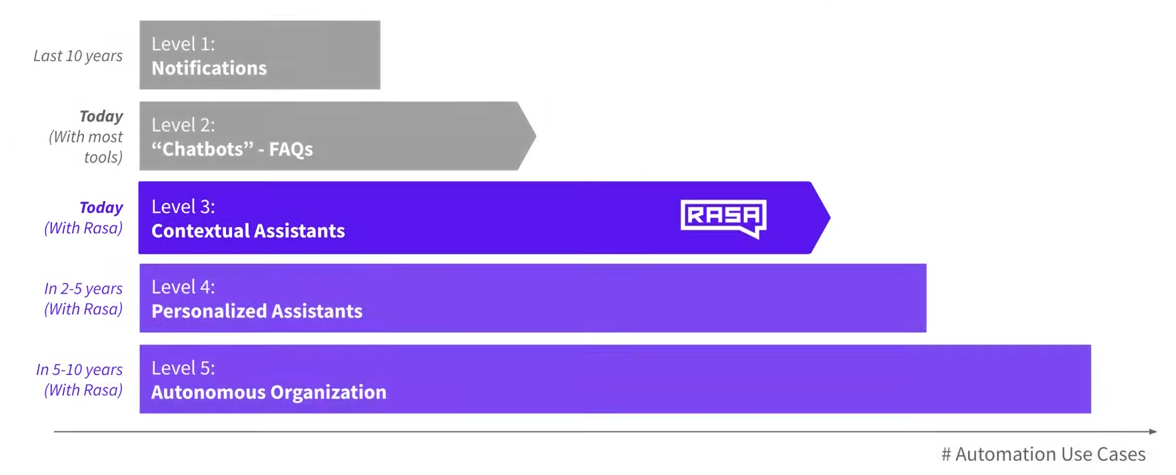
\includegraphics[scale=0.25]{pics/5_levels_of_ai}
    \caption{5 Stufen von AI~\cite{ai5LevelsVideo}}
    \label{fig:5_levels_of_ai}
\end{figure}

\textbf{Level 1: Notifications}

Auf Level 1 geht es darum, simple Aufgaben zu erfüllen, wie man sie möglicherweise von seinem Smartphone kennt.
Darunter fällt zum Beispiel das Anlegen von Terminen und anderen Benachrichtigungen, die man dann zu einer eingestellten Uhrzeit bekommt.\cite{rasaMasterclass5Levels,ai5Levels,ai5LevelsVideo}

\textbf{Level 2: "Chatbots" \& FAQs}

Auf Level 2 geht es darum, dass die Benutzerin oder der Benutzer einfache Fragen stellen kann und anschließend der Chatbot auf diese antwortet.
Diese Art von Chatbots findet man sehr oft, allerdings sind diese sehr fehleranfällig, weil hier nur eine Menge an Regeln angelegt wird, an die sich der Chatbot hält.
Dies wird sehr oft in Form von FAQs genutzt und auch ein paar kleine Follow-up Fragen können hierbei schon definiert sein.\cite{rasaMasterclass5Levels,ai5Levels,ai5LevelsVideo}

\textbf{Level 3: Contextual AI Assistants}

Dieses Level wird derzeit von Rasa unterstützt.
Zusätzlich zu normalen FAQs wird hierbei auch der Kontext beachtet.
Es macht nämlich einen Unterschied, wann, wie und in welcher Situation ein Benutzer etwas gesagt hat.
Bei Contextual Assistants wird der Kontext also was bereits zuvor gesagt wurde, auch beachtet.
Außerdem lenken sie Konversationen in die gewünschte Richtung und werden mit der Zeit immer besser, wenn man sie trainiert.\cite{rasaMasterclass5Levels,ai5Levels,ai5LevelsVideo}

\section{Komponenten}\label{sec:components}
\setauthor{Lukas Starka}

In der sogenannten Domain werden alle Intents ~\ref{subsec:Intents}, Entities ~\ref{subsection:entities}, Slots ~\ref{subsec:slots}, Responses ~\ref{subsec:Responses}, Forms ~\ref{subsection:forms} und Actions ~\ref{subsec:actions} angegeben, die der Bot kennt.
Diese ganzen Informationen befinden sich in der \textbf{domain.yml} Datei.\cite{domain}

\subsection{Intents}\label{subsec:Intents}
\setauthor{Lukas Starka}

Intents sind die Absichten hinter der Nachricht des Benutzers.
Als Intents werden also alle möglichen Beispielsätze definiert, die ein Benutzer sagen könnte, um eine bestimmte Absicht auszudrücken.\cite{intents}

Intents werden in der \textbf{nlu.yml} Datei wie in Listing ~\ref{lst:intent-example} angegeben:

\begin{lstlisting}[label={lst:intent-example},caption={Intents Beispiel}]{Intents Beispiel}
## intent:<name des intents>
- <phrase 1>
- <phrase 2>
- <phrase 3>
\end{lstlisting}

\subsection{Responses}\label{subsec:Responses}
\setauthor{Lukas Starka}

Responses sind die Antworten, die vom Bot gegeben werden, wenn ein bestimmter Intent erkannt wurde.\cite{responses}

Responses fügt man in der \textbf{domain.yml} Datei in der Form, wie in Listing ~\ref{lst:responses-example} gezeigt, ein.

\begin{lstlisting}[label={lst:responses-example},caption={Responses Beispiel}]{Responses Beispiel}
responses:
  utter_<name der response>:
  - text: "<text>"
    image: "<img link>"
    buttons:
    - title: "<button title>"
      payload: "<payload>"
  ...

z.B.

utter_chitchat/what_are_you_doing:
    - text: Ach nichts besonderes, nur ein wenig chatten!
    - text: Ich entspanne gerade ein wenig aber durchlöcher mich ruhig mit Fragen ich muss sowieso wieder an die Arbeit.
    - text: Frag mich ruhig etwas ich brauche sowieso eine Ablenkung von all dem was ich eigentlich machen sollte!
      buttons:
        - title: "Wie geht es dir?"
          payload: "Wie geht es dir?"
        - title: "Willst du mich heiraten?"
          payload: "Willst du mich heiraten?"
        - title: "Welche Technologien wurden für dich verwendet?"
          payload: "Welche Technologien wurden für dich verwendet?"
        - title: "Wie spät ist es?"
          payload: "Wie spät ist es?"
\end{lstlisting}

\subsection{Stories}\label{subsec:Stories}
\setauthor{Lukas Starka}

Stories werden als Trainingsdaten verwendet, die zum Trainieren des Modells des Bots verwendet werden.
Stories können dabei genutzt werden, um Modelle zu trainieren, bei denen auch unvorhersehbare Konversationspfade behandelt werden und die sich unterscheiden von den Rules ~\ref{subsec:Rules}.\cite{stories}

Bei einer Story wird also die Unterhaltung zwischen einem Benutzer und dem Bot dargestellt.
Dabei wird die Eingabe des Benutzers als Intent ~\ref{subsec:Intents} angegeben und die Antwort, mit der der Bot antworten soll, als Name der Action ~\ref{subsec:actions}.\cite{stories}

Stories können wie in Listing ~\ref{lst:stories-example} aufgezeigt aussehen und sind in der \textbf{stories.yml} Datei anzugeben:

\begin{lstlisting}[label={lst:stories-example},caption={Stories Beispiel}]{Stories Beispiel}
stories:
- story: name der story
  steps:
  - intent: <name des intents>
  - action: <name der action>

z.B.
stories:
  - story: sad path 1
    steps:
      - intent: greet
      - action: utter_greet
      - intent: mood_unhappy
      - action: utter_cheer_up
      - action: utter_did_that_help
      - intent: affirm
      - action: utter_happy
\end{lstlisting}

\subsubsection{Checkpoints und OR-Statements}\label{subsubsec:Checkpoints}

Stories können außerdem mit Checkpoints und OR-Statements versehen werden.
Bei diesen sollte aber grundsätzlich aufgepasst werden und diese sollten nur bedacht verwendet werden, weil in den meisten Fällen die gewünschten Resultate besser mit \textbf{Rules} ~\ref{subsec:Rules} oder einem \textbf{ResponseSelector} ~\ref{subsec:response-selector} zu erzielen sind.\cite{checkpointsor}

Checkpoints können genutzt werden, um seine Trainingsdaten zu vereinfachen, indem ein Checkpoint in einer Story gesetzt wird und auf diesen in einer anderen Story wieder angesetzt wird.
Von diesen sollte man allerdings nicht zu viele machen, weil sonst die Stories sehr leicht schwer zu lesen und unübersichtlich sind und außerdem die Trainingszeit dadurch erhöht wird.\cite{checkpoints}

Ein Checkpoint wird am Ende der Story definiert, wenn dieser Teil der Story auch wieder als Voraussetzung für eine weitere Story gesetzt sein soll.
In der nächsten Story wird dann mit dem Checkpoint, also dem Punkt, auf den angeknüpft wird, begonnen.

In Listing ~\ref{lst:checkpoints-example} werden Checkpoints von Stories verwendet, um an anderen Stories anzuknüpfen\cite{checkpoints}:

\begin{lstlisting}[label={lst:checkpoints-example},caption={Checkpoints Beispiel}]{Checkpoint Beispiel}
stories:
- story: beginning of flow
  steps:
  - intent: greet
  - action: action_ask_user_question
  - checkpoint: check_asked_question

- story: handle user affirm
  steps:
  - checkpoint: check_asked_question
  - intent: affirm
  - action: action_handle_affirmation
  - checkpoint: check_flow_finished

- story: handle user deny
  steps:
  - checkpoint: check_asked_question
  - intent: deny
  - action: action_handle_denial
  - checkpoint: check_flow_finished

- story: finish flow
  steps:
  - checkpoint: check_flow_finished
  - intent: goodbye
  - action: utter_goodbye
\end{lstlisting}

OR-Statements können dafür verwendet werden, wenn man auf mehrere Intents innerhalb einer Story gleich reagieren möchte.\cite{orStatements}

Hierbei wird also anstelle von einem Intent in der Story ein \textbf{or} geschrieben und darunter werden alle Intents angegeben, von denen einer eintreffen muss, damit die Story zutrifft.

\begin{lstlisting}[label={lst:or-example},caption={OR Beispiel}]{OR Beispiel}
stories:
- story:
  steps:
  # ... vorherige schritte
  - action: utter_ask_confirm
  - or:
    - intent: affirm
    - intent: thankyou
  - action: action_handle_affirmation
\end{lstlisting}

\subsection{Rules}\label{subsec:Rules}
\setauthor{Lukas Starka}

Rules werden angegeben, um kleine Teile von Unterhaltungen anzugeben, die immer wieder gleichbehandelt werden sollen.
Diese sollten allerdings nicht allzu häufig verwendet werden, weil nie alle Konversationen vorhergesagt werden können.
Um Rules verwenden zu können, muss die \textbf{RulePolicy} in der Policy Konfiguration eingetragen sein.\cite{rules}

Eine Rule wird wie in Listing ~\ref{lst:rules-example} beschrieben, in der Datei \texttt{rules.yml} angegeben.

\begin{lstlisting}[label={lst:rules-example},caption={Rules Beispiel}]{Rules Beispiel}
rules:

- rule: Say `hello` whenever the user sends a message with intent `greet`
  steps:
  - intent: greet
  - action: utter_greet
\end{lstlisting}

\subsection{Slots}\label{subsec:slots}
\setauthor{Lukas Starka}

Slots sind sozusagen das Gedächtnis des Bots.
Diese sind als Key-Value-Paare dargestellt und können dazu verwendet werden, damit Information, die der Benutzer bereitstellt, gespeichert werden können, ähnlich zu Entities.
Diese Informationen können beispielsweise der Name des Benutzers sein oder Informationen, die für den generellen Kontext des Gesprächs wichtig sind.\cite{slots}

\begin{lstlisting}[label={lst:slots-example},caption={Slots Beispiel}]{Slots Beispiel}
slots:
  slot_name: <slot name>
    type: <type>

z.B.

slots:
  name:
    type: rasa.shared.core.slots.TextSlot
    initial_value: null
    auto_fill: true
    influence_conversation: false
\end{lstlisting}

\subsection{Entities}\label{subsection:entities}
\setauthor{Lukas Starka}

Entities sind strukturierte Stücke von Informationen, die sich innerhalb der Nachricht eines Benutzers befinden.
Solche Entities können beispielsweise ein Ort, ein Beruf oder ein Name sein.\cite{entities}

Entities werden wie in Listing ~\ref{lst:entities-domain-example} in der Datei \texttt{domain.yml} angegeben.

\begin{lstlisting}[label={lst:entities-domain-example},caption={Entities in der Domain}]{Entities in der Domain}
entities:
  - <entity name>
  - <entity name>

z.B.

entities:
  - name
  - branch
  - teacher
  - class
  - grade
  - subject
\end{lstlisting}

Diese Entities müssen dann noch in den Intents angegeben werden, in denen sie vorkommen sollen.
Dies wird dadurch erreicht, dass folgende Syntax von Listing ~\ref{lst:entities-nlu-example} bei den Trainingssätzen in der \textbf{nlu.yml} Datei ergänzt wird.

\begin{lstlisting}[label={lst:entities-nlu-example},caption={Entities Beispiel}]{Entities Beispiel}
Hallo mein Name ist [Lukas](name).
Ich hätte gerne eine [kleine](size) [Pizza](meal)
\end{lstlisting}

\subsubsection{Entity Roles}\label{subsubsec:entity-roles}

Entity Roles können sinnvoll in manchen Szenarien sein.

\begin{lstlisting}[label={lst:entity-roles-example},caption={Entity Roles Beispiel}]{Entity Roles Beispiel}
Buche einen Flug von [Linz](city) nach [London](city).
\end{lstlisting}

In dem Fall von ~\ref{lst:entity-roles-example} sind sowohl Linz als auch London zwar richtig gekennzeichnet als Entity mit dem Namen \texttt{city}, allerdings reicht diese Information noch nicht aus, damit der Chatbot richtig reagieren kann.
Hierbei wäre es praktisch, wenn noch angegeben wird, welche dieser zwei Städte das Ziel und welche der Abflugort ist.
Mithilfe von Entity Rules kann dies erzielt werden.\cite{entityRolesGroups}

\subsubsection{Entity Groups}\label{subsubsec:entity-groups}

Entity Groups können genutzt werden, wenn Entities miteinander gruppiert werden sollen.\cite{entityRolesGroups}

Im Beispiel von ~\ref{lst:entity-groups-example} kann dies von Vorteil sein.

\begin{lstlisting}[label={lst:entity-groups-example},caption={Entity Groups Beispiel}]{Entity Groups Beispiel}
Ich hätte gerne eine kleine [Pizza](meal) mit [Pilzen](topping) und eine [Salami](topping) [Pizza](meal).
\end{lstlisting}

Bei der Gruppe muss hier erkannt werden, welche zwei Entities zusammen gehören\cite{entityRolesGroups}:

\begin{lstlisting}[label={lst:entity-groups-example-2},caption={Entity Groups Beispiel 2}]{Entity Groups Beispiel 2}
Ich hätte gerne eine kleine [Pizza](meal) mit [Pilzen](topping) und eine [Salami](topping) [Pizza](meal).
Group 1: [Pizza](meal) [Pilzen](topping)
Group 2: [Salami](topping) [Pizza](meal)
\end{lstlisting}

Um Entity Groups oder Entity Roles nutzen zu können, muss in der Pipeline entweder der CRFEntityExtractor ~\ref{subsec:crfentityextractor} oder der DIETClassifier ~\ref{subsec:dietclassifier} verwendet werden.
Diese sind die einzigen Entity Extraktoren, die Role und Group Labels erkennen können.\cite{entityRolesGroups}

\subsection{Forms}\label{subsection:forms}
\setauthor{Lukas Starka}

Um mehrere Informationen von einem Benutzer zu bekommen, eignen sich Forms.
Um Forms zu verwenden, muss die \textbf{RulePolicy} in der Policy Konfiguration eingetragen sein.\cite{forms}

Wenn ein Formular hinzugefügt werden soll, muss dies in der forms Sektion in der \textbf{domain.yml} Datei angegeben sein.

\begin{lstlisting}[label={lst:forms-example},caption={Forms Beispiel}]{Forms Beispiel}
forms:
  restaurant_form:
    required_slots:
        cuisine:
          - type: from_entity
            entity: cuisine
        num_people:
          - type: from_entity
            entity: number
\end{lstlisting}

\subsection{Synonyms}\label{subsection:synonyms}
\setauthor{Lukas Starka}

Mithilfe von Synonymen können extrahierten Entities einen anderen Wert annehmen, als sie eigentlich vorher hatten, wenn diese in der Bedeutung gleich sind.
Wenn also mit verschiedenen Wörtern dasselbe gemeint ist, können Synonyme zur Hilfe genommen werden.\cite{synonyms}

Ein Beispiel dafür wäre ~\ref{lst:synonym-example} in der \textbf{nlu.yml} Datei.

\begin{lstlisting}[label={lst:synonym-example},caption={Synonym Beispiel}]{Synonym Beispiel}
- synonym: Medientechnik
  examples: |
    - IT-Medientechnik
    - IT Medientechnik
    - Medientechnologie
\end{lstlisting}

\subsection{Actions}\label{subsec:actions}
\setauthor{Lukas Starka}

Es gibt 2 verschiedene Arten von Messages:

\begin{enumerate}
    \item \textbf{Static Messages}: Diese sind unabhängig vom User Input und benötigen keinen Action Server\cite{actionsVid}
    \item \textbf{Dynamic Messages}: Diese sind abhängig vom User Input und benötigen einen Action Server ~\ref{subsec:custom-actions}\cite{actionsVid}
\end{enumerate}

Der Rasa Action Server führt sogenannte Custom Actions ~\ref{subsec:custom-actions} für einen Rasa Open Source Conversation Assistent aus.

Wenn der Assistant eine gewisse Custom Action vorhersagt, sendet der Rasa Server einen POST-Request an den Actionserver mit einer JSON Payload mit dem Namen der vorhergesagten Action, der Conversation ID, den Inhalten des Trackers und den Inhalten der Domain.\cite{actions}

\subsection{Custom Actions}\label{subsec:custom-actions}
\setauthor{Lukas Starka}

Neben normalen Responses können auch Custom Actions definiert werden.
Diese sind in Python zu schreiben und dabei kann eigener Code für Berechnungen oder dergleichen verwendet werden.
Hierbei muss eine Klasse implementiert werden, die Kind der Klasse \texttt{Action} ist und eine Methode \texttt{name} und \texttt{run} besitzt.
Eine Custom Action wird beim Leobot beispielsweise für die Ausgabe des aktuellen Datums genutzt, wie bei Listing ~\ref{lst:custom-date-action} zu sehen ist.

\begin{lstlisting}[label={lst:custom-date-action},caption={Custom Action für die Ausgabe des aktuellen Datums}]{Custom Action}
class ActionWhatDateIsIt(Action):
    def name(self) -> Text:
            return "action_what_date_is_it"

    def run(self, dispatcher: CollectingDispatcher,
            tracker: Tracker,
            domain: Dict[Text, Any]) -> List[Dict[Text, Any]]:

        now = datetime.now()
        weekday = datetime.today().weekday()
        weekday_string = ("Montag", "Dienstag", "Mittwoch", "Donnerstag", "Freitag", "Samstag", "Sonntag")[weekday]

        current_date = now.strftime("%d.%m.%Y")
        print("Current Date =", current_date)

        dispatcher.utter_message(text=f"Heute ist {weekday_string} der {current_date}!")

        return []
\end{lstlisting}

Nun muss die Custom Action in der \textbf{domain.yml} Datei definiert werden, wie in Listing ~\ref{lst:domain-custom-action} zu sehen ist.

\begin{lstlisting}[label={lst:domain-custom-action},caption={Custom Actions in Domain definiert}]{Custom Action Domain}
actions:
  - action_what_date_is_it
\end{lstlisting}

\section{Initialisieren}\label{section:initialize}
\setauthor{Lukas Starka}

\subsection{Rasa Init}\label{subsec:rasa-init}
\setauthor{Lukas Starka}

Ein neuer Rasa Assistant kann mithilfe des Init-Befehls in der Konsole erstellt werden.
Der Befehl dafür lautet, wie in Listing ~\ref{lst:init-example} zu sehen ist.

\begin{lstlisting}[language=bash,label={lst:init-example},caption={Befehl fürs Initialisieren}]{Rasa Init Befehl}
rasa init
\end{lstlisting}

Bei diesem Befehl wird man gefragt, ob man direkt ein voreingestelltes Modell trainieren möchte.
Dieses Modell wird basierend auf den Demodaten, die von jedem neu erstellten Rasa Projekt zur Verfügung gestellt werden, trainiert.

\begin{figure}[hbt!]
    \centering
    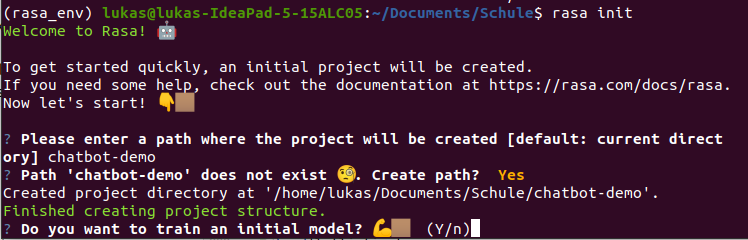
\includegraphics[scale=0.5]{pics/rasa_init}
    \caption{Rasa Init Konsolenausgabe}
    \label{fig:rasa_init}
\end{figure}

Danach wird eine Struktur, wie in Abbildung ~\ref{fig:file_tree} erzeugt.

\begin{figure}[hbt!]
    \centering
    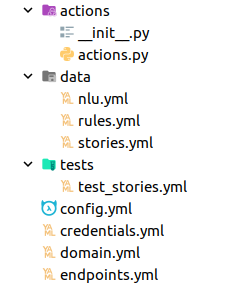
\includegraphics[scale=0.75]{pics/rasa_file_tree}
    \caption{File Tree nach dem Initialisieren}
    \label{fig:file_tree}
\end{figure}


\section{Trainieren}\label{section:train}
\setauthor{Lukas Starka}

\subsection{Rasa Train}\label{subsec:rasa-train}
\setauthor{Lukas Starka}

Um das Modell nun zu trainieren, wird der \texttt{Rasa train} Befehl benützt.
Dabei werden nur die Komponenten (Core ~\ref{subsec:rasa-core} oder NLU ~\ref{subsec:rasa-nlu}) trainiert, die sich auch geändert haben im Vergleich zu dem letzten Modell.
Es kann aber auch selbstständig angeben werden, dass nur \texttt{core} oder \texttt{nlu} trainieren werden soll.
Nach dem Trainieren wird das Modell in den Pfad gespeichert, der beim \texttt{--out} definiert wurde und standardmäßig \texttt{/models} ist.
Dabei wird als Modellname der aktuelle Zeitstempel gewählt, außer es wird die \texttt{--fixed-model-name} Flag verwendet.
Wenn andere Pipelines oder Policies verwendet werden sollen, kann auch eine andere config-Datei angegeben werden, in dem diese gespeichert sind.
Dies wird mit \texttt{-c} erreicht.
Ab Rasa 2.2 gibt es außerdem die Möglichkeit eine Feinabstimmung an einem bereits bestehenden Modell vorzunehmen.
Dies macht man, wenn man neue Trainingsdaten bei bereits bestehenden Intents hinzugefügt hat.
Hierbei ergibt sich eine viel kürzere Trainingszeit, als wenn das Modell noch einmal von vorne trainiert würde und dabei wird der Pfad zum Modell angegeben, wenn nicht, wie standardmäßig definiert, das neueste trainiert werden soll.\cite{rasaTrain}

\begin{lstlisting}[language=bash,label={lst:rasa-train},caption={Rasa Train Befehle}]{Rasa Train}
rasa train
rasa train -c config.yml #Das verwendete Config File (default: config.yml)
rasa train --out trained-models/ #Der Pfad, in dem das Modell gespeichert wird (default: models/)
rasa train --fixed-model-name leobot-model #Der Name des Modells (default: <timestamp>.tar.gz)
rasa train core #Rasa Core mit den Stories trainieren
rasa train nlu #Rasa NLU mit den NLU-Daten trainieren
rasa train --finetune models/20220211-094939.tar.gz #Finetune eines bestehenden Modells
\end{lstlisting}


\section{Interagieren}\label{sec:interact}
\setauthor{Lukas Starka}

\subsection{Rasa Shell}\label{subsec:rasa-shell}
\setauthor{Lukas Starka}

Wenn man sich nun mit seinem Bot unterhalten möchte, kann man eine ChatSession über die Konsole mit dem \texttt{rasa train} Befehl.
Normalerweise wird dabei das aktuellste Modell genommen.
Allerdings kann auch mit der \texttt{--model} Flag auch der Pfad zum richtigen Modell angegeben werden.

\begin{lstlisting}[language=bash,label={lst:shell-command},caption={Rasa Shell Befehle}]{Rasa Shell}
rasa shell
rasa shell --model models/20220211-094939.tar.gz #Das Modell, das verwendet werden soll
rasa shell --debug #Debug-Modus aktivieren
\end{lstlisting}

Für detailliertere Ausgaben kann außerdem die \texttt{--debug} Flag verwendet werden.
Die Ausgabe dabei sieht wie in Abbildung ~\ref{fig:rasa_shell} aus:

\begin{figure}[hbt!]
    \centering
    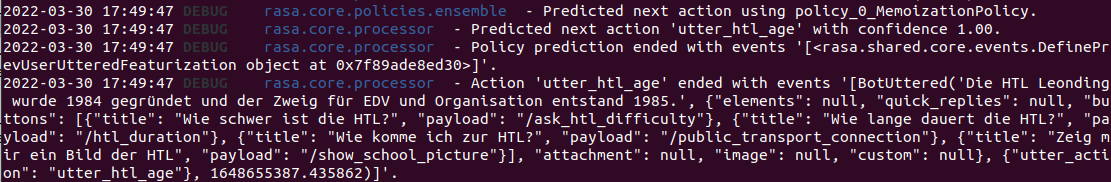
\includegraphics[scale=0.40]{pics/rasa_shell}
    \caption{Rasa Shell Ausgabe mit Debug Flag}
    \label{fig:rasa_shell}
\end{figure}

\subsection{Rasa Interactive}\label{subsec:rasa-interactive}
\setauthor{Lukas Starka}

Um eine interaktive Session mit dem Bot zu starten, kann der Befehl \texttt{rasa interactive} genutzt werden.
Dabei wird zunächst ein Modell trainiert und anschließend startet eine interaktive Shell Session.
Dabei hat die Benutzerin oder der Benutzer die Möglichkeit, alle vorhergesagten Aktionen vom Assistant zu korrigieren.
Wenn nur das Core Modell getestet werden soll, kann dies spezifiziert werden.

\begin{lstlisting}[language=bash,label={lst:interactive-command},caption={Interaktive Trainingssession starten}]{Rasa Interactive}
rasa interactive
rasa interactive --model models/20220211-094939.tar.gz #Das Modell, das verwendet werden soll
rasa interactive core #Interaktive Session für das Core Modell starten
\end{lstlisting}

Bei dieser Trainingssession hat man die Möglichkeit, jedes Mal anzugeben, ob der vorhergesagte Intent und die daraus resultierende Antwort die Richtige sind.
Außerdem wird die gesamte Chat History visualisiert und ausgegeben, wie in Abbildung ~\ref{fig:rasa_interactive} zu sehen ist.

\begin{figure}[hbt!]
    \centering
    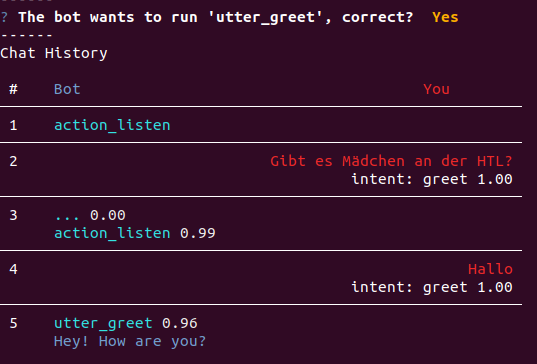
\includegraphics[scale=0.80]{pics/rasa_interactive}
    \caption{Ausgabe beim Interactive Befehl}
    \label{fig:rasa_interactive}
\end{figure}
